\documentclass[12pt]{article}
\usepackage[margin = 1 in]{geometry}
\usepackage{amsmath, amsfonts, graphicx, amsthm}

\newcommand{\F}{\mathbf{F}}
\newcommand{\C}{\mathbb{C}}
\newcommand{\R}{\mathbb{R}}
\renewcommand{\P}{\mathbb{P}}
\newcommand{\GL}{\mathrm{GL}}
\newcommand{\A}{\mathbb{A}}
\newcommand{\Aff}{\mathrm{Aff}}
\renewcommand{\vec}{\overrightarrow}

\newtheorem{fact}{Fact}
\newtheorem{definition}{Definition}
\newtheorem{example}[]{Example}
\newtheorem{theorem}{Theorem}

\title{Algebraic Geometry Notes}
\author{Raman Aliakseyeu}
\date{Winter 2024}

\begin{document}
    \maketitle
    \noindent \textbf{Course by Daniil Rudenko.} \par 
    We will start with projective geometry, and then add algebra to it. No schemes in this course, we will be closer to the 19th century stuff. We are not following any particular book(s). Number one book is "Algebraic Geometry" by Shafarevich, our goal is all of chapter 1. We will start with projective geometry, a book for that is (on canvas). 
    \section{Projective Geometry} 
    \subsection{Lecture 1} 
        Algebraic geometry studies solutions to systems of algebraic equations/algebraic curves (which are loci of solutions of algebraic equations). One of the most famous renaissance geometry results is the Pascal theorem: the points $G, H, I$ in the diagram below are colinear for any configuration of $A, B, C, D, E, F$ on the circle. 
        \begin{center}
            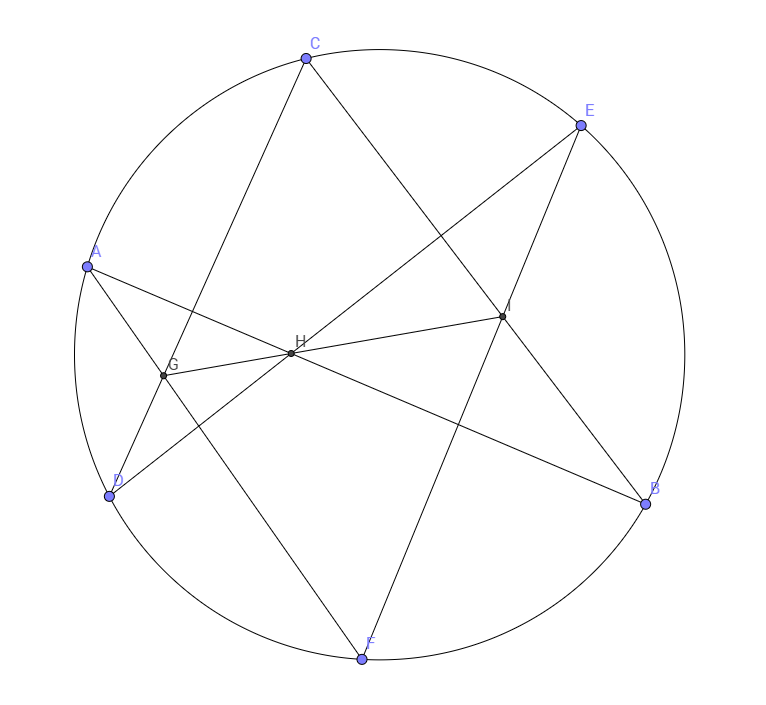
\includegraphics[width = 0.5 \linewidth]{pascals-theorem.PNG}
        \end{center}
        A similar result to that is Pappus' theorem. Another top theorem is by Cayley-Salman 1849: A smooth projective cubic surface contains exactly 27 lines. Another such theorem is that any smooth projective curve of degree 4 has 28 bitangent lines (tangent in exactly two points). Working toward proofs of these results using algebraic geometry is our goal. \par 
        \textit{History of the subject}: throughout the 19th century it developed very quickly, people who were into Euclidean geometry just transitioned to algebraic geometry and discover miracles like we described above. During the late 19th century Italians, who before led algebraic geometry, started producing very incorrect results because the technical aspects became too hard. Oscar Zariski and others saved the subject by rigorizing it using commutative algebra, with the language of ideals and rings, etc. We will see some `wrong' arguments by the Italian school and see why they are not precise enough. There was another revolution by Grothendieck and the Bourbaki group in developing the language of schemes, which we will not touch in this course (``You will need to sacrifice a year of your life to start speaking that language. I never needed to, but a lot of people do.'')\par 
        (Rudenko plug: woollymathematics.com)\par 
        Take $\F$ to be some field (usually $\C$), and polynomials $p_1, \dots, p_k \in \F[x_1, \dots, x_n]$, and study the solutions to the system 
        $$\begin{cases}
            p_1(x_1, \dots, x_n) = 0 \\
            \vdots \\
            p_k(x_1, \dots, x_n) = 0
        \end{cases}$$
        \begin{fact}
            If $k = 1$ and $p_1(x) = x^d + a_{d-1}x^{d-1} + \dots + a_0$ for $d \geq 1$, $p_1(x) = 0$ has $\leq d$ solutions in $\F$. 
        \end{fact}
        If $k = 2$, the number of solutions is $\leq$ than the product of the degrees of the polynomials. Of course we usually want a precise number of solutions, but generally we can't hope for anything more than upper bounds. 
        \begin{fact}
            If $\F = \C$, then $p(x) = 0$ has a solution. 
        \end{fact}
        This is a remarkably hard result called the Fundamental Theorem of Algebra. There is a result that is in a way easier:
        \begin{fact}
            If $\F = \C$, then $p(x) = 0$ has exactly $d$ solutions if counted with multiplicity. 
        \end{fact} 
        We would hope for something like that but for $k > 1$. Bezoiut's theorem kind of satisfies that, but the picture is more complicated. For example, take a line and a hyperbola. While we would expect $4$ solutions up to multiplicity, but take a line intersecting one of the components of the hyperbola transversally that is parallel to one of the other component's asymptotes. However, everything becomes nicer if we change the complex plane to the projective plane. The study of geometry on the projective plane is the projective geometry, and that's what we will study first. \par 
        \begin{definition} \label{def:proj_plane}
            Let $\F$ be a field. A \textbf{projective space} $\P_\F^n$ is the set of lines in the vector space $\F^{n+1}$. 
        \end{definition}
        An example for $\F = \R$, $\P_{\R}^2$ is the set of lines through the origin in the real plane. We can think of $\P_\R^1$ as all the points of a line in $\R^2$ not through the origin (say the line $y = 1$ in $\R^2$) but with a point at infinity added. \par 
        In $\R^2$, usually two lines intersect at one point, and two points are contained in one line. We can also define $\P_\R^2$ as the set of points of $\R^2$, and the set $[l]$ (points at $\infty$), which are equivalence classes of lines in $\R^2$ by $l_1 \sim l_2$ for $l_1$ and $l_2$ are parallel. Note that there is one more line, line at infinity, consisting only of points $[l]$. \par 
        \begin{fact}
            In $\P^2_\R$ every two distinct lines intersect in one point and every two points are contained in precisely one line. 
        \end{fact}
        \begin{proof}
            Non-parallel lines intersect in the usual way. Parallel lines intersect at their equivalence class $[l]$. If one of the lines is the `line at infinity', they intersect at the equivalence class of the other line. Similarly we can examine the second part of the statement. 
        \end{proof}
        \begin{fact}
            For $\P_\R^2$, the abstract definition \ref{def:proj_plane} is equivalent to the definition we gave in the example. 
        \end{fact}
        \begin{proof}
            Take a plane in $\R^3$ not passing through the origin, $z = -1$ for example. Then we can create a bijection between the set of lines through the origin and the set of points on the plane and the set of points at infinity, by mapping the lines that intersect the plane with their intersection point, and those that are parallel with the plane to their equivalence class on the plane $\R^2$. Thus we have a bijection between the two objects we defined. 
            \begin{center}
                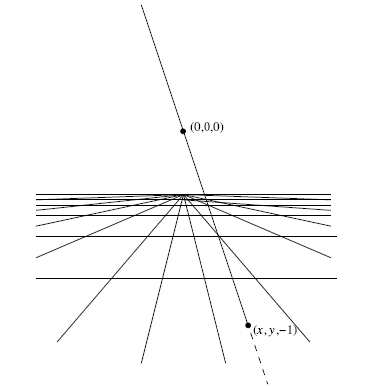
\includegraphics[width = 0.4\linewidth]{proj-plane.jpg}
            \end{center}
        \end{proof}
        Another way to think of $\P_\R^2$ is as a sphere with antipodal points identified. \par
        ``ChatGPT can make you Snake 4: Snake but on the projective plane.''
        
    \subsection{Lecture 2}
    (OH Wednesday 5PM)\par 
    A \textbf{geometry} is a set $X$ along with a group $G$ acting on $X$, $x \mapsto gx$, which defines `equivalences' between subsets of $X$. 
    \begin{example}
        \begin{itemize}
            \item Let $X = \R^2$, $G$ the group of \textbf{isometries}: distance preserving bijections. Indeed, isometries also preserve lengths, areas, angles, etc. Think of them as congruences in Euclidean geometry. 
            \item Let $X$ be a vector space, $G = \text{GL}(V)$, the general linear group. More specifically, let $X = F^n$ for some field $G$, then $G = \GL_n(F)$.  
        \end{itemize}
    \end{example}
    \begin{definition}
        Fix $F$ some field. Define \textbf{affine space} $\A_F^n = F^n$, with the group of \textbf{affine transformations} $$\mathrm{Aff}_n = \{f: \A^n \to \A^n \mid f(x) = Ax + b, A \in \GL_n(F), b \in A^n\}$$
    \end{definition}
    A typical way of thinking about affine space is as a vector space without a fixed origin. 
    \begin{example}
        Circles don't make much sense in $\A_\R^2$ anymore, since $x^2 + y^2 = 1$ is equivalent to an ellipse (say by $(x, y) \mapsto (2x, 5y)$). 
    \end{example}
    \begin{definition}
        An \textbf{affine algebraic variety} is a set of solutions of a system of polynomials $P_1, \dots, P_k \in F[x_1, \dots, x_n]$:
        $$\begin{cases}
            P_1(x_1, \dots, x_n) = 0 \\
            \vdots \\
            P_k(x_1, \dots, x_n) = 0
        \end{cases}$$
    \end{definition}
    \begin{example}
        \begin{itemize}
            \item $P_1(x, y) = 2x + y - 1 = 0$ gives a line; $P_1(x, y) = x^2 + y^2 - 1 = 0$ gives a circle.
            \item $P_1(x, y, z) = 2x+y-z-1 = 0$ and $P_2(x, y, z) = x + y -3 = 0$, then the variety is an intersection of two planes, thus a line.  
        \end{itemize}
    \end{example}
    If $P_1, \dots, P_k$ are linear $\sum a_i x_i + b$ then we will call it \textbf{affine subspace}.\par 
    We can identify pairs of points in $\A^n$ with vectors in a vector space $F^n$, where vectors $\overrightarrow{AB}$ are pairs of points $(A, B)$, identified via the equivalence relation $\overrightarrow{A_1B_1} \sim \overrightarrow{A_2B_2}$ iff $(A_1)_i - (B_1)_i = (A_2)_i - (B_2)_i$. An observation is that if $f: \A^n \to \A^n$ is an affine transformation, then $f(\overrightarrow{AB}) = \overrightarrow{f(A)f(B)}$. \par 
    What we just described is a homomorphism $\mathrm{Aff}_n \to \GL_n$ which maps $f = Ax + b$ to $A \in \GL_n$. The kernel of this map is isomorphic to $\F^n$ as an additive group. \par 
    \begin{definition}
        If $A_1, \dots, A_{n+1} \in \A^n$ are in \textbf{general position} if $\overrightarrow{A_1A_i}$ for $i = 2, 3, \dots n+1$ are all linearly independent. Equivalently (exercise) $A_1, \dots, A_{n+1}$ are not in the same affine hyperplane. 
    \end{definition}
    \begin{theorem}
        Suppose $A_1, \dots, A_{n+1} \in \A^n$ and $B_1, \dots, B_n \in \A^n$ are points in general position in $\A^n$. Then there is a unique $f \in \Aff_n$ s.t. $f(A_i) = B_i$ for each $i$.  
    \end{theorem}
    \begin{proof}
        [Proof sketch:] Using translation by a vector $\overrightarrow{A_1B_1}$, move $A_1$ to $B_1$. This reduces this problem to the uniqueness of a linear transformation from the basis $\overrightarrow{A_1A_i} \to \overrightarrow{B_1B_i}$. 
    \end{proof}
    Observation: ``$X$ is the midpoint of the segment $\overline{A_1A_2}$'' is an affine property: $f(X)$ is still the midpoint of $\overline{f(A_1)f(A_2)}$. Application of this: 
    \begin{theorem}
        Three medians of a triangle intersect at a point. 
    \end{theorem} 
    \begin{proof}
        Let $ABC$ be an arbitrary triangle in $\A_\R^2$. Let $f$ be the affine transformation taking an equilateral triangle to $ABC$. The medians of an equilateral triangle intersect at a point by symmetry. But medians get sent to medians, and intersections are preserved, so the medians of $ABC$ must intersect also. 
    \end{proof}
    \begin{definition}
        Let $V$ be a vector space over $F$, then its \textbf{projectivization} $\P(V)$ is the set of lines (1-dim vector subspaces) in $V$. 
    \end{definition}
    By definition the dimension of $\P(V)$ is $\dim V - 1$. If $V = F^{n+1}$, $\P(V) = \P_F^n$. More explicitly, $\P(V) = (V - \{0\})/(v \sim \lambda v, \lambda \in F)$. 
    We express points in $\P(V)$ by \textbf{homogeneous coordinates} so $[X_0: X_1 : \dots : X_n]$, with the aforemetioned equivalence relation (so e.g. $[0, 1, 0] = [0, 2, 0]$) \par 
    ``Gold to silver to whiskey, the ratio should be 1 to 1 to 100. You're making a cocktail. Don't do that by the way... Point of projective geometry is to make cocktails.''\par 
    If $A = [X_0: \dots :X_n] \in \P^n$. If $X_n \neq 0$ then $A = [X_0/X_n: \dots : X_{n-1}/X_n, 1]$, points of this form this are in bijection with $\A^n$. Indeed, $\P^n = \A^n \sqcup \A^{n-1} \sqcup \dots \sqcup \A^0$. The points with $X_n = 0$ are in bijection with points in $\P^n$ (divide all entrees by the first non-zero entry from the right). For example, $\P_\R^1 = \R \cup \infty$, where $\R$ is in bijection with points $[X_0/X_1:1]$ and $\infty$ represents $[1:0]$.  \par 
    \textbf{Barycentric coordinates} are basically the same thing as homogeneous coordinates but in a different language. Imagine putting masses $m_1, m_2, m_3$ at the vertices of a triangle, then look at their center of mass. If $m_1 = m_2 = m_3$ then this point is the centroid. More precisely, if $O$ is any point, we have that $M$, the center of mass for some $m_1, m_2, m_3$ (sum non-zero) is
    $$\vec{OM} = \frac{m_1\vec{OA_1} + m_2\vec{OA_2} + m_3\vec{OA_3}}{m_1 + m_2 + m_3}$$
    If we put this triangle onto $\R^3$ with vertices at $(1:0:0)$, $(0:1:0)$, $(0:0:1)$, then the center of mass of $m_1, m_2, m_3$ with respect to the origin will have homogeneous coordinates $[m_1:m_2:m_3]$. \par 
    A homogeneous polynomial is one where each term has the same degree. Then it makes sense to talk about $P([x_0, \dots, x_d]) = 0$ for a homogeneous polynomial $P$, since such polynomials respect the equivalence relation of homogeneous coordinates. 
    \begin{definition}
        \textbf{Projective variety} is a subset of $\P_F^n$ which is the set of solutions of a system:
        $$\begin{cases}
            P_1([X_0: \dots : X_n]) = 0 \\ 
            \vdots \\
            P_k([X_0: \dots : X_n]) = 0
        \end{cases}$$
        where each $P_i$ is homogeneous. 
    \end{definition}
    \begin{example}
        Say $P(x, y, z) y - x^2$, which we can think of as points $[x:y:1]$ that satisfy the parabola. We can relabel $[x:y:1]$ into $[X:Y:Z]$ with $x = X/Z, y = Y/Z$, so the set of points satisfying $P_1([X:Y:Z])$ is the set such that $X^2 = YZ$. So for instance $[0:1:0]$ is also a solution. We can think of this as the parabola becoming an ellipse because it closes at infinity. 
    \end{example}

\end{document} 